\documentclass[12pt]{article}

\usepackage[utf8x]{inputenc} % Включаем поддержку UTF8  
\usepackage[russian]{babel}  % Включаем пакет для поддержки русского языка  
\usepackage{hyperref}        % Для гиперссылок

% Математика
\usepackage{amsmath,amsfonts,amssymb,amsthm,mathtools} % AMS
\usepackage{icomma}
\usepackage{mathrsfs}

% Прога
\usepackage{etoolbox}
\usepackage{listings}

% Цвета
\usepackage{xcolor}

% Картинки
\usepackage{graphicx}
\graphicspath{ {./images/} }

\usepackage{tikzsymbols}

% Работа с таблицами
\usepackage{array,tabularx,tabulary,booktabs} % Дополнительная работа с таблицами
\usepackage{longtable}  % Длинные таблицы
\usepackage{multirow} % Слияние строк в таблице

\newtheorem{property}{Свойство}
\newtheorem{consequence}{Следствие}[property]

\begin{document}

\thispagestyle{empty}
\begin{center}
\textbf{ПРАВИТЕЛЬСТВО РОССИЙСКОЙ ФЕДЕРАЦИИ}

\vspace{5ex}
	
\textbf{Федеральное государственное автономное образовательное учреждение \\ высшего образования \\ <<Национальный исследовательский университет \\ <<Высшая школа экономики>>}
\end{center}
\vspace{5ex}

\begin{center}
    Московский институт электроники и математики им. А.Н. Тихонова  
    
    \vspace{5ex}
    
    Департамент прикладной математики
    
    \vspace{10ex}
    \textbf{Отчёт \\ по лабораторной работе №2 \\ по курсу <<Компьютерный практикум>> \\ Вариант №7}
	\vspace{7ex}

\end{center}

\begin{center} 
\begin{tabular}{| p{0.3\linewidth}| p{0.3\linewidth}| p{0.3\linewidth}|}
 \hline	
ФИО студента & Номер группы & Дата \\  \hline
 & & \\  
Вязов Глеб \newline Дмитриевич & БПМ-231 & 07.01.2024\\  
 & & \\  \hline		
\end{tabular}
\end{center}

\begin{center}
	\vspace{3ex}
	
	\vfill
   
   \normalsize
    
	\textbf{Москва, 2023}
\end{center}

\newpage

%---------------------------------------------------------------------------------

\section*{Задание}\addcontentsline{toc}{section}{Введение}
Вычислить с помощью ассемблерной вставки:

 $$\upsilon = \frac{x(y+5)-3}{z-4}+3$$
 
 $$x=2h, y=-7h, z=-3h, \upsilon = 4h$$
 $$x=3FB5h, y=7Dh, z=-7Eh, \upsilon = -3FB1h$$
 $$y, z - \text{байты}; x, \upsilon - \text{слова}$$

\newpage

%---------------------------------------------------------------------------------

\section*{Решение}\addcontentsline{toc}{section}{Решение}
\lstset{ %
texcl=true,%
language=C,                 % выбор языка для подсветки
basicstyle=\small\sffamily, % размер и начертание шрифта для подсветки кода
numbers=left,               % где поставить нумерацию строк (слева\справа)
numberstyle=\tiny,           % размер шрифта для номеров строк
stepnumber=1,                   % размер шага между двумя номерами строк
numbersep=5pt,                % как далеко отстоят номера строк от подсвечиваемого кода
backgroundcolor=\color{white}, % цвет фона подсветки - используем \usepackage{color}
showspaces=false,            % показывать или нет пробелы специальными отступами
showstringspaces=false,      % показывать или нет пробелы в строках
showtabs=false,             % показывать или нет табуляцию в строках
frame=single,              % рисовать рамку вокруг кода
tabsize=3,                 % размер табуляции по умолчанию равен 2 пробелам
captionpos=t,              % позиция заголовка вверху [t] или внизу [b] 
breaklines=true,           % автоматически переносить строки (да\нет)
breakatwhitespace=false, % переносить строки только если есть пробел
escapeinside={\%*}{*)},   % если нужно добавить комментарии в коде
inputencoding=utf8x,
extendedchars=\true
}

\begin{lstlisting}[label=string_code1,caption=C]
#include <stdio.h>
#include <windows.h>

short int assembly(short int x, char y, char z) {
    short int v = 0;

    __asm__(".intel_syntax noprefix \n" // Меняем синтаксис AT T на синтаксис Intel
            // Вычисляем знаменатель
            "mov al, %3             \n" // al = z              (байт)
            "cbw                    \n" // ax = al             (слово)
            "mov bx, ax             \n" // bx = ax             (слово)
            "sub bx, 4              \n" // bx = bx - 4         (слово)                        (z - 4)
            // Вычисляем числитель
            "mov al, %2             \n" // al = y              (байт)
            "cbw                    \n" // ax = al             (слово)
            "add ax, 5              \n" // ax = ax + 5         (слово)                        (y + 5)
            "imul %1                \n" // dx = ax * x         (двойное слово)                x(y + 5)
            "sub ax, 3              \n" // ax = ax - 3         (слово, младшее слово)
            "sbb dx, 0              \n" // dx = dx - 0         (двойное слово, старшее слово) x(y + 5) - 3
            // Вычисляем дробь
            "idiv bx                \n" // ax = dx / bx        (слово)                        x(y + 5) - 3 / (z - 4)
            "add ax, 3              \n" // ax = ax + 3         (слово)
            "mov %0, ax             \n" // v = ax              (слово)
            ".att_syntax prefix;    \n"
            : "=r"(v)                // выходной оператор v --> %0
            : "r"(x), "r"(y), "r"(z) // входное оператор x --> %1, y --> %2, z --> %3
            : "eax"
            );

    return v;
}

int main() {
    // Меняем кодировку на UTF-8, чтобы можно было писать на русском
    SetConsoleOutputCP(CP_UTF8);
    // Объявление переменных. Дружественный интерфейс
    printf("Выполнил задание: Вязов Глеб. Группа: БПМ231\n");

    char y, z; // байты
    short int x, v; // слова

    x = 0x2, y = -0x7, z = -0x3;
    v = ((x*(y+5) - 3) / (z-4)) + 3; // v=0x4
    short int res = assembly(x, y, z);

    printf("Первый тест: \n");
    printf("x=%d, y=%d, z=%d\n", x, y, z);
    printf("Ответ на C: v(10)=%d | v(16)=%xh \n", v, v);
    printf("Ответ на ассемблере: v(10)=%d | v(16)=%xh \n", res, res);

    x = 0x3FB5, y = 0x7D, z = -0x7E;
    v = ((x*(y+5) - 3) / (z-4)) + 3; // v=-0x3FB1
    res = assembly(x, y, z);

    printf("\nВторой тест: \n");
    printf("x=%d, y=%d, z=%d\n", x, y, z);
    printf("Ответ на C: v(10)=%d | v(16)=%xh \n", v, v);
    printf("Ответ на ассемблере: v(10)=%d | v(16)=%xh \n", res, res);
}
\end{lstlisting} 

\section*{Тестирование}\addcontentsline{toc}{section}{Тестирование}

    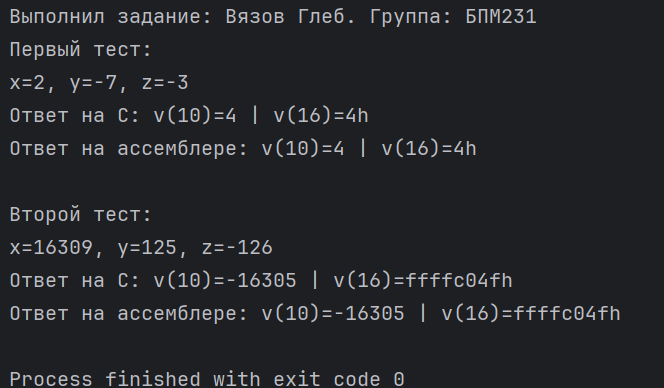
\includegraphics[width=\linewidth]{img1}

\end{document}
